
%(BEGIN_QUESTION)
% Copyright 2008, Tony R. Kuphaldt, released under the Creative Commons Attribution License (v 1.0)
% This means you may do almost anything with this work of mine, so long as you give me proper credit

Studer følgende grafer, som viser trykk langs strømningsbanen i tre ulike reguleringsventiler:

$$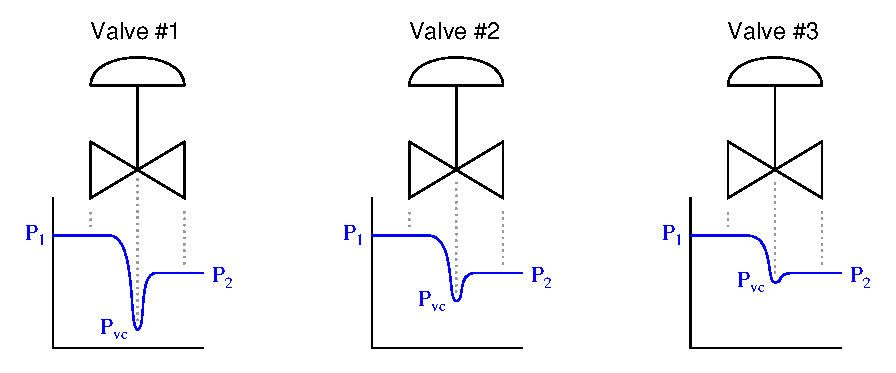
\includegraphics[width=15.5cm]{i01418x01.eps}$$

Som du ser av grafene, er innløpstrykkene ($P_1$) og utløpstrykkene ($P_2$) de samme for hver ventil. Med andre ord har alle tre ventilene samme permanente trykkfall. Men hva som skjer inne i hver ventil er ganske forskjellig, noe som vises ved de ulike {\it vena contracta}-trykkene ($P_{vc}$).

Når væsken går inn i en innsnevret del av ventilen, øker hastigheten. Høyere væskehastighet betyr at væskemolekylene har høyere kinetisk energi enn før. I henhold til energibevaringsloven må denne økningen i kinetisk energi balanseres av tilsvarende tap i potensiell energi (væsketrykk) gjennom innsnevringen. Dette forklarer det brå trykkfallet ved vena contracta-punktet (punktet med maksimal innsnevring inne i ventilen).  

Etter innsnevringen går væsken inn i en bredere del av ventilen og senker farten. Molekylær kinetisk energi avtar mens potensiell energi (trykk) øker. Derfor ``henter'' trykket seg inn igjen nedstrøms for vena contracta. Differansen mellom oppstrøms- og nedstrømstrykk ($P_1 - P_2$) representerer væskeenergi som tapes i ventilens struping.

\vskip 10pt

Bestem hvilken av de tre ventilene som har størst {\it trykkgjenvinning}, og hvilken av de tre som har størst {\it trykkgjenvinningsfaktor} (ofte kalt {\it pressure recovery coefficient}). Bestem deretter hvilken av de tre ventilene som er mest utsatt for kavitasjon i væskeservice, alt annet likt.

Til slutt: Oppgi ventiltyper som kjennetegnes av ytterpunkter for trykkgjenvinning og trykkgjenvinningsfaktor.

\underbar{file i01418}
%(END_QUESTION)





%(BEGIN_ANSWER)

{\it Trykkgjenvinning} er trykkforskjellen mellom utløpstrykket ($P_2$) og vena contracta-trykket ($P_{vc}$):

$$\hbox{Trykkgjenvinning} = P_2 - P_{vc}$$

$$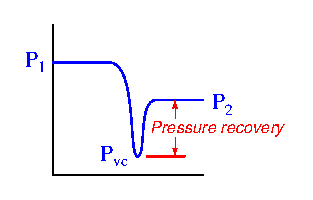
\includegraphics[width=15.5cm]{i01418x02.eps}$$

{\it Trykkgjenvinningsfaktor} beregnes ved å dividere det permanente trykkfallet med trykkfallet fra innløp ($P_1$) til vena contracta ($P_{vc}$):

$$F_L = \sqrt{{P_1 - P_2} \over {P_1 - P_{vc}}}$$

Basert på denne definisjonen har ventil \#1 størst trykkgjenvinning og lavest $F_L$, og er dermed mest utsatt for kavitasjon. For å unngå eller redusere kavitasjon er det best å bruke en reguleringsventil med lav trykkgjenvinning (høy $F_{L}$-faktor). Roterende ventildesign som kule-, skive- og spjeldventiler har vanligvis større trykkgjenvinning (lavere $F_{L}$-tall) enn globeventiler, og er derfor mer utsatt for kavitasjon.

\vskip 10pt

Ironisk nok har reguleringsventiler med lav trykkgjenvinning høye $F_L$-verdier. Omvendt har ventiler med høy trykkgjenvinning lave $F_L$-verdier. For å unngå eller redusere kavitasjon er det best å bruke en reguleringsventil med lav trykkgjenvinning (stor $F_{L}$-faktor). Alt annet likt (oppstrøms- og nedstrømstrykk, strømningsrate, spesifikk vekt osv.) vil en ventil med stor $F_{L}$ ha høyere vena contracta-trykk ($P_{vc}$) enn en ventil med liten $F_{L}$.

\vskip 10pt

Roterende ventildesign (kule, skive, spjeld osv.) har vanligvis større trykkgjenvinning (mindre $F_{L}$-tall) enn globeventiler, noe som gjør dem mer utsatt for kavitasjon. Grunnen til denne større trykkgjenvinningen er den relativt rette og brede strømningsbanen gjennom ventilhuset før og etter strupeelementet. Globeventiler, med mer kroket strømningsbane, gir større trykkfall over hele ventilhuset. Dermed trenger ikke plugg/sete-åpningen i en globeventil gjøre {\it alt} arbeidet med å redusere prosessvæskens trykk.

Ved samme totale trykkfall ($P_1 - P_2$) vil trimmet i en globeventil gi mindre trykkfall enn trimmet i en tilsvarende roterende ventil med samme $C_{v}$. Dette gir høyere vena contracta-trykk ($P_{vc}$) inne i globeventilen, og gjør den mindre utsatt for flashing og kavitasjon enn en tilsvarende roterende ventil.

\filbreak

Illustrasjonen under viser forskjellen i strømningsbaner mellom en spjeldventil og en globeventil. Her ser du hvordan globeventildesignet ikke er avhengig av at plugg/sete-innsnevringen er {\it eneste} punkt for trykkfall, slik tilfellet er i spjelddesign:
 
$$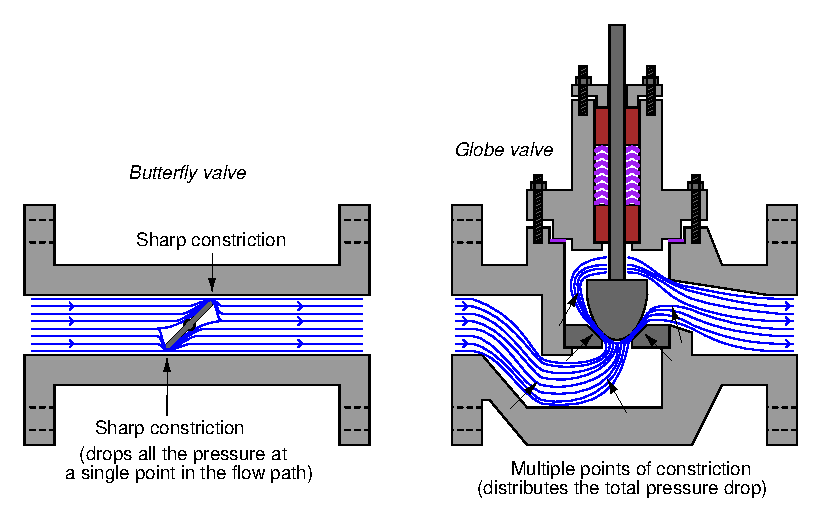
\includegraphics[width=15.5cm]{i01418x03.eps}$$

\vskip 10pt

$F_L$ endrer seg med ventilspindelposisjon, akkurat som $C_v$. For ventiler med høy $F_L$, som globeventiler, er endringen i $F_L$ gjennom ventilslaget liten. For ventiler med lav $F_L$, som spjeldventiler, er endringen i $F_L$ mye større fra helt åpen til helt stengt.

\vskip 10pt

Ventiltrim utformet for å redusere kavitasjon oppnår typisk svært høye (nær 1) $F_L$-verdier. For Fishers Cavitrol-trim er oppgitt $F_L$-verdi 0.98 for totrinns trim og 0.99 for tretrinns trim, noe som betyr at $P_{vc}$ er svært nær lik $P_2$ (nedstrøms).

\vskip 10pt

\filbreak

Oppfølgingsspørsmål: Studer illustrasjonene under og forklar deretter {\it hvorfor} roterende ventildesign som spjeld- og kuleventiler har lavere $F_L$-verdier enn globeventiler i sammenlignbar størrelse:

$$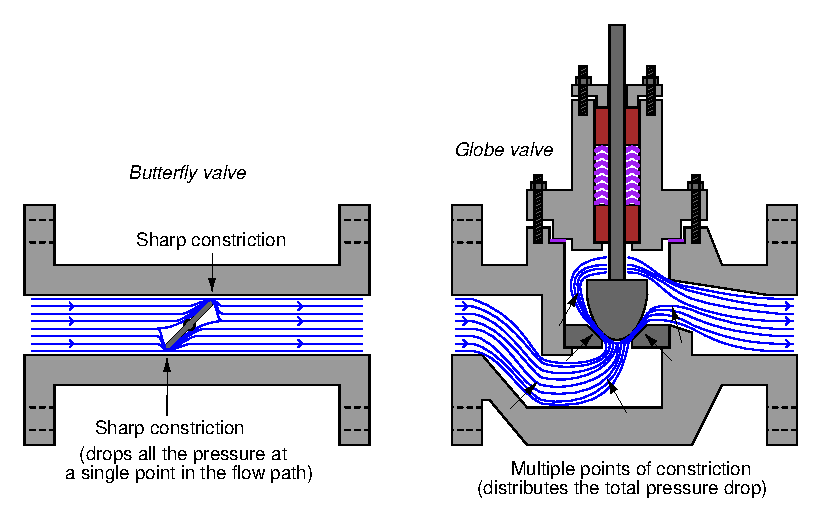
\includegraphics[width=15.5cm]{i01418x03.eps}$$

%(END_ANSWER)





%(BEGIN_NOTES)


%INDEX% Final Control Elements, valve: cavitation control
%INDEX% Final Control Elements, valve: pressure recovery coefficient
%INDEX% Final Control Elements, valve: pressure recovery factor

%(END_NOTES)

